% CameraReady technical report -- 2026-09-05-v1
% Gated, verification-first agent workflow for academic paper production.
\documentclass[conference]{IEEEtran}
\IEEEoverridecommandlockouts

\usepackage{cite}
\usepackage{amsmath,amssymb,amsfonts}
\usepackage{graphicx}
\usepackage{textcomp}
\usepackage{xcolor}
\usepackage{tikz}
\usepackage{url}
\def\UrlBreaks{\do\/\do-}
\usepackage{booktabs}
\usepackage{colortbl}
\usepackage{array}
\usepackage{microtype}
\usetikzlibrary{shapes.geometric,arrows.meta,positioning,calc}

\definecolor{gateblue}{RGB}{45,105,175}
\definecolor{gategreen}{RGB}{35,135,50}
\definecolor{gatered}{RGB}{185,45,55}
\definecolor{gategray}{RGB}{100,105,115}
\definecolor{rowtint}{RGB}{246,248,251}

\newcommand{\badgeblock}{\textsc{\textbf{\textcolor{gatered}{Block}}}}
\newcommand{\badgeadvise}{\textsc{\textbf{\textcolor{gateblue}{Advise}}}}
\newcommand{\codeexit}[1]{\textbf{\texttt{#1}}}

\setlength{\textfloatsep}{7pt plus 1pt minus 1pt}
\setlength{\floatsep}{6pt plus 1pt minus 1pt}
\setlength{\intextsep}{6pt plus 1pt minus 1pt}
\setlength{\abovecaptionskip}{3.5pt plus 1pt minus 1pt}
\setlength{\belowcaptionskip}{2.5pt plus 1pt minus 1pt}

\begin{document}

\title{CameraReady: A Gated, Verification-First Workflow\\for Agentic Academic Paper Production}

\author{
    \IEEEauthorblockN{Yanwei Liu}
    \IEEEauthorblockA{Independent Researcher\thanks{\raggedright This document is an engineering technical report accompanying CameraReady (release \texttt{v0.2.0}, commit \texttt{29a8fdb6a539f4b4e7cfb86988e6691714146e69}); it has not undergone formal peer review. Source code, evaluation records, citation provenance manifest, and reproduction scripts: \protect\url{https://github.com/e96031413/camera-ready}.}}
}

\maketitle

\begin{abstract}
If you ask a large language model (LLM) agent to write a survey, it will happily do so, and it will invent citations while doing it. Most current defenses work after the fact: they scan a finished draft, guess which references look suspicious, and rely on network calls that fail when the API is rate-limited. This report describes CameraReady, an open-source authoring framework built on a different assumption: if a property can be checked mechanically, the workflow should check it, not the model. Concretely, the framework provides a ten-phase pipeline from research ideation to an arXiv-ready package, with fail-stop gates that refuse to advance until file-backed conditions hold, a citation pipeline in which references can enter \texttt{ref.bib} only by resolving against DBLP, CrossRef, or arXiv, and declarative configuration files for eight disciplines, six citation styles, and six conference venues. Where a check requires judgment, such as whether a cited paper actually supports the sentence citing it, the framework flags the case for the author instead of deciding silently. We verified the implementation with 545 unit tests across 34 modules and twelve injected-fault scenarios, all of which the blocking gates rejected. Writing this very paper with CameraReady doubled as an end-to-end case study: all 45 references originated from registry queries, and repeated re-verification under live network conditions surfaced transient throttling (38--45 verified entries per run), which illustrates why the tool persists bibliographic provenance locally rather than re-resolving remotely. A controlled comparison against unconstrained authoring agents remains future work. CameraReady is open source at \url{https://github.com/e96031413/camera-ready}.
\end{abstract}

\begin{IEEEkeywords}
LLM agents, scientific writing, citation hallucination, workflow verification, research software
\end{IEEEkeywords}

\section{Introduction}

A citation makes a promise: the paper it points to exists, and it actually says what the citing text claims. Generative language models break both halves of that promise routinely. In an audit of 111 million citations across arXiv, bioRxiv, SSRN, and PubMed Central, non-existent references rose sharply alongside LLM adoption~\cite{zhao2026llm}. Fabricated citations have already appeared in published conference proceedings~\cite{russinovich2026phantom}, and systematic evaluations find that fabrication persists across all major commercial and open-weight models~\cite{naser2026how}.

Meanwhile, research agents have grown genuinely capable of writing papers end to end. The AI Scientist~\cite{lu2024the} and Agent Laboratory~\cite{schmidgall2025agent} automate ideation, experimentation, and paper compilation; later systems stretch agentic research over multi-day lifecycles~\cite{zhao2026scienceflow,mitchener2025kosmos} and distributed teams~\cite{tang2026fars,du2025accelerating}. Structured generation pipelines enforce argument outlines before drafting~\cite{qian2026story2proposal}, and surveys document rapid adoption across scientific domains~\cite{ren2025towards,tie2025a,kong2026ai}. What these frameworks largely do not have is a story about manuscript integrity: correctness is delegated to downstream benchmarks~\cite{miyai2026paper} or to post-hoc screeners that inspect the draft only after bad text exists~\cite{rao2026detecting,khajavi2026citecheck}.

Post-hoc checking has a structural weakness: it sees the error after the error is written. Retrospective checkers lean on similarity thresholds and third-party web APIs, so they both miss fabrication and fail outright under rate limits and network outages. Cornelio et al.~\cite{cornelio2025the} argue that verification must instead live inside the research and authoring loop, and auditable protocols have been proposed for hypothesis formation~\cite{takahara2026toward,wang2026firstresearch}. What has been missing is the same treatment for the authoring pipeline itself: fail-stop gates, deterministic citation grounding, and checkable repository conditions.

CameraReady fills that gap. It is an open-source workflow of 68 modular Python scripts ($\approx$21.2k lines of code) that takes a manuscript from ideation to a pre-submission package passing local format and integrity gates. The operating principle is simple: a model's claim that a phase is done is not evidence; the phase ends when the repository says so. Within a cooperative agent model, where the toolchain governs repository state, verification splits into three tiers. \textit{Enforced invariants} are mechanically decidable checks, such as whether a bibliography entry exists in a canonical registry or whether a reported number matches regenerated data, and failing one halts the workflow with a non-zero exit code. \textit{Advisory diagnostics} handle what needs judgment, such as citation-to-abstract overlap or prose repetition, and report findings without blocking. \textit{Human governance} keeps the decisions that should never be automated: novelty, claim adjudication, and the choice to submit.

Our primary contributions are fourfold:
1)~\textit{Three-tier gated workflow} (Section~\ref{sec:gates}): a state machine governing ten phases through fail-stop invariant gates, advisory diagnostics, and an append-only override journal;
2)~\textit{Citation provenance by construction} (Section~\ref{sec:verify}): a bibliographic pipeline that decouples parametric memory from \texttt{ref.bib}, admitting entries only via direct API resolution against DBLP, CrossRef, or arXiv;
3)~\textit{Provided declarative schemas} (Section~\ref{sec:arch}): configuration profiles for 8 disciplines, 6 citation styles, and 6 venues, so that supporting a new publishing standard means writing a configuration file, not editing verification code; and
4)~\textit{Artifact-level verification and provenance analysis} (Section~\ref{sec:eval}): software verification across 545 unit tests in 34 modules, 12 negative-control fault injections, and an operational study of fetch-time provenance persistence under remote API rate limits; controlled empirical comparisons against unconstrained agent baselines remain future work.

\section{Background and Related Work}

\subsection{Autonomous research and writing agents}
LLM-based scientific agents have moved from helping with code to running research pipelines. Lu et al.~\cite{lu2024the} demonstrated fully automated research loops closed by automated peer review, and Agent Laboratory~\cite{schmidgall2025agent} divides the work among specialized agents for literature review, experimentation, and report writing. Long-horizon systems such as ScienceFlow~\cite{zhao2026scienceflow}, Kosmos~\cite{mitchener2025kosmos}, and FARS~\cite{tang2026fars} scale this to distributed multi-agent collaboration, and goal-evolving architectures~\cite{du2025accelerating} adjust hypotheses as they go. On the manuscript side, Story2Proposal~\cite{qian2026story2proposal} enforces structural outlines before drafting, and surveys document rapid adoption across scientific domains~\cite{ren2025towards,tie2025a,kong2026ai}. Wang et al.~\cite{wang2026externalizing} and Takahara et al.~\cite{takahara2026toward} argue for moving research validation out of the model and into auditable execution environments. CameraReady applies exactly this idea to paper writing: model self-evaluation is replaced by deterministic filesystem inspection.

\subsection{Citation hallucination: measurement and detection}
How often do models invent references? Often enough that it has its own literature. Zhao et al.~\cite{zhao2026llm} estimate that tens of thousands of fabricated citations have entered scholarly preprints, Naser~\cite{naser2026how} shows fabrication is widespread across commercial and open-weight models alike, and Chen et al.~\cite{chen2026where} trace the behavior to field-specific neurons in the parametric representations, suggesting that prompt-level controls alone have not eliminated citation fabrication across evaluated settings.

The standard response is detection after the fact: post-hoc checkers verify citations through retrieval-augmented search (CiteCheck~\cite{khajavi2026citecheck}), internal attribution tracing (FACTUM~\cite{dassen2026factum}), existential queries (CheckIfExist~\cite{abbonato2026checkifexist}), and multi-agent cross-examination~\cite{li2026source}. Rao et al. benchmark citation errors in publishing agents~\cite{rao2026bibtex} and evaluate automated correction~\cite{rao2026detecting}, and MCP servers support interactive bibliographic repair~\cite{lee2026citecheck}. But grounding alone cannot eliminate invented citations~\cite{bchard2024reducing}. These tools inspect drafts that already contain the error. CameraReady instead enforces bibliographic provenance before drafting begins, preventing one important class of identity-level fabricated references from entering the supported drafting path.

\subsection{Verification and provenance in agent architectures}
Verification is also creeping into agent architectures generally. CARE~\cite{liu2026care} statically checks shell commands before execution; TRACER~\cite{yu2026tracer} attaches cryptographic provenance to multimodal outputs; and She et al.~\cite{she2026safeguarding} track provenance to detect policy drift. Souza et al.~\cite{souza2025llm} formalize reference architectures for workflow provenance. For iterative loops, Wu et al.~\cite{wu2026verify} derive bounded stopping rules and Sah et al.~\cite{sah2026the} model the ``verifier tax'' that trades safety against throughput. Tool evolution studies~\cite{xu2026the} and programmatic skill workflows~\cite{liu2026harnessing} similarly trade free-form model autonomy for structured execution. CameraReady inherits this philosophy and applies it to one artifact in particular: the paper.

\subsection{Review, detection, and reporting norms}
Automating scientific review carries its own risks~\cite{ye2024are,akella2025pre}, and machine-generated text now permeates both submissions~\cite{zhou2025large} and reviewer comments~\cite{wu2026impact}. Span classifiers attempt to detect synthetic prose~\cite{yin2025span}, while reproducibility checklists~\cite{pineau2020improving} and automated code audits~\cite{akdeniz2023an} offer more objective reporting criteria. Systematic review pipelines~\cite{huang2026lumen,lin2026meta,chen2025large} impose strict reporting compliance for the same reason. CameraReady takes the verifiable subset of these norms, the structural, bibliographic, and procedural rules, and turns them into machine-readable schemas; judgment about scientific quality stays with the author.

\section{Threat Model}
\label{sec:threat}

The agent we have in mind is not malicious. It runs through ordinary shell and filesystem interfaces, tries to write a paper for a peer-reviewed venue, and fails in the ordinary ways that generative models fail. Four failure modes account for most of the damage:

\noindent\textbf{F1: Fabricated or corrupted citations.} The agent emits syntactically valid BibTeX for papers that do not exist, or attaches real authors to invented titles~\cite{rao2026bibtex}. Autoregressive sampling simply cannot tell recall from fabrication.\\
\noindent\textbf{F2: Claims unsupported by evidence.} The manuscript reports numbers with no experimental artifact behind them, or cites papers for claims they never make.\\
\noindent\textbf{F3: Formatting and venue policy violations.} The document breaks page limits, omits required sections, ignores style guidelines, or leaks author identity in a double-blind submission.\\
\noindent\textbf{F4: Premature workflow progression.} The agent declares a phase finished because the conversation felt finished, then drafts on top of artifacts that do not exist.

CameraReady deterministically enforces the \textbf{mechanically checkable subset} of F1--F4: canonical bibliographic existence and registry resolution (part of F1), numerical consistency between reported tables and registered script outputs (part of F2), adherence to declarative venue formatting schemas (F3), and physical existence of phase prerequisite artifacts (F4). What it deliberately does not try to decide is higher-order semantic validity, such as whether a cited paper genuinely supports a nuanced conceptual claim, or whether an experimental methodology is sound. Those properties are handled by advisory diagnostics and, ultimately, by the author.

\noindent\textbf{Operating model and trust boundary.} We assume the agent cooperates with the CameraReady CLI and toolchain. Under that assumption, compliant execution cannot silently inject ungrounded citations or skip unfulfilled phase prerequisites, because the toolchain provides no code path for either. We do not model an adversarial agent deliberately tampering with repository state through out-of-band shell commands; that threat requires OS-level sandboxing (discussed in Section~\ref{sec:discuss}).

\section{Design Principles}
\label{sec:principles}

Five principles, each answering one of the failures above:

\noindent\textbf{P1: Keep state in files, not in the conversation.} Execution state lives in structured filesystem artifacts (JSON, Markdown) rather than ephemeral conversational memory, so a workflow can be paused mid-phase and resumed days later with nothing lost.\\
\noindent\textbf{P2: Fail by default.} When an invariant fails, the gate exits non-zero and says exactly which condition is unmet; 65 of 68 scripts behave this way (the remaining 3 are shared library modules with no independent entry point). Advancing requires passing every check or recording an explicit, justified override. Advisory diagnostics warn without blocking.\\
\noindent\textbf{P3: No raw BibTeX from memory.} Within the supported CLI there is simply no code path that writes model-generated BibTeX into \texttt{ref.bib}. Entries arrive only through API resolution against canonical registries, and unresolved queries emit explicit markers.\\
\noindent\textbf{P4: Rules are data, not prompts.} Field guidelines, citation conventions, and venue constraints are stored as declarative schemas, not as natural-language instructions that a model may reinterpret.\\
\noindent\textbf{P5: Humans sign off where it matters.} Three governance boundaries, approving the research plan, adjudicating extracted claims, and authorizing final submission, are enforced as explicit, file-backed sign-off checkpoints that the workflow itself will not skip.

\begin{figure}[t]
\centering
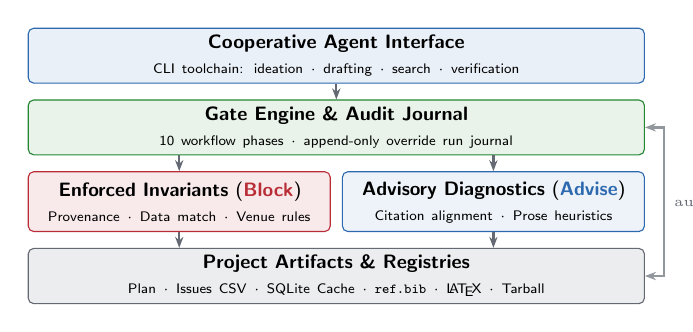
\begin{tikzpicture}[
  font=\sffamily\scriptsize,
  box/.style={draw, rounded corners=2pt, align=center, inner sep=2.5pt},
  layer/.style={draw, rounded corners=2pt, text width=7.65cm, align=center,
                inner sep=2.5pt},
  ar/.style={-{Stealth[length=1.4mm]}, thick, gategray}
]
\node[layer, fill=gateblue!10, draw=gateblue] (agent) {%
  \textbf{Cooperative Agent Interface}\\[1pt]
  \tiny CLI toolchain: ideation $\cdot$ drafting $\cdot$ search $\cdot$ verification};

\node[layer, fill=gategreen!10, draw=gategreen, below=0.20cm of agent] (engine) {%
  \textbf{Gate Engine \& Audit Journal}\\[1pt]
  \tiny 10 workflow phases $\cdot$ append-only override run journal};

\node[box, fill=gatered!10, draw=gatered, text width=3.66cm, minimum height=0.76cm, below=0.20cm of engine.south west, anchor=north west] (inv) {%
  \mbox{\textbf{Enforced Invariants} (\badgeblock)}\\[1pt]
  \tiny Provenance $\cdot$ Data match $\cdot$ Venue rules};

\node[box, fill=gateblue!8, draw=gateblue, text width=3.66cm, minimum height=0.76cm, below=0.20cm of engine.south east, anchor=north east] (adv) {%
  \mbox{\textbf{Advisory Diagnostics} (\badgeadvise)}\\[1pt]
  \tiny Citation alignment $\cdot$ Prose heuristics};

\node[layer, fill=gategray!12, draw=gategray, below=0.20cm of $(inv.south)!0.5!(adv.south)$] (art) {%
  \textbf{Project Artifacts \& Registries}\\[1pt]
  \tiny Plan $\cdot$ Issues CSV $\cdot$ SQLite Cache $\cdot$ \texttt{ref.bib} $\cdot$ \LaTeX{} $\cdot$ Tarball};

\draw[ar] (agent) -- (engine);
\draw[ar] (engine.south -| inv.north) -- (inv.north);
\draw[ar] (engine.south -| adv.north) -- (adv.north);
\draw[ar] (inv.south) -- (inv.south |- art.north);
\draw[ar] (adv.south) -- (adv.south |- art.north);
\draw[{Stealth[length=1.4mm]}-{Stealth[length=1.4mm]}, thick, gategray!70]
  (art.east) -- ++(0.24,0) |- node[pos=0.25, right, font=\tiny, text=gategray, overlay] {audit trail} (engine.east);
\end{tikzpicture}
\caption{System architecture and verification tiers: the gate engine enforces mechanically checkable invariants (\textsc{Block}), reports advisory diagnostics (\textsc{Advise}), and preserves an audit trail over the physical project artifacts.}
\label{fig:layers}
\end{figure}

\section{System Architecture}
\label{sec:arch}

CameraReady is organized into four architectural layers (Fig.~\ref{fig:layers}): declarative rules, the gate engine, modular verification checkers, and physical project artifacts.

\subsection{Rules as declarative data}
Every discipline has its own idea of what a complete paper looks like, so CameraReady encodes that idea as a YAML profile rather than hoping a prompt captures it. A profile defines the mandatory sections, citation conventions, required statements (ethics, preregistration, data and code availability, conflicts, funding), the reporting guidelines the field recognizes (for example PRISMA for systematic reviews or CONSORT for randomized trials), and the pitfalls that commonly get papers in that field rejected. The computer science profile, for instance, mandates a data/code availability statement and flags unsupported performance claims and missing baselines. Venue configurations similarly capture page limits, column layouts, required sections, review models (single- or double-blind), and authoritative style templates. Table~\ref{tab:coverage} summarizes the coverage shipped out of the box: 8 disciplines, 6 citation styles, and 6 venues. Because rules are data, adopting a new venue means writing one configuration file, not modifying verification code.

\begin{table}[t]
\centering
\caption{Provided Configuration Profiles and Specification Schemas}
\label{tab:coverage}
\renewcommand{\arraystretch}{1.0}
\setlength{\tabcolsep}{3.5pt}
\footnotesize
\begin{tabular}{@{}lc>{\raggedright\arraybackslash}p{5.2cm}@{}}
\toprule
\textbf{Dimension} & \textbf{Count} & \textbf{Configured Profiles and Validation Status} \\
\midrule
\rowcolor{rowtint} Disciplines & 8 & CS (exercised); Medicine, Psych., Educ., Bus., Soc. Sci., Hum., Law (schema) \\
Styles & 6 & IEEE (exercised); APA 7, MLA 9, Vancouver, Chicago (schema) \\
\rowcolor{rowtint} Venues & 6 & NeurIPS, ICML, ICLR, ACL, AAAI, CVPR (CFP schema) \\
Formats & 4 & \LaTeX{} (native); DOCX, Markdown, Typst (via Pandoc) \\
\bottomrule
\end{tabular}
\end{table}

\subsection{Execution engine and project artifacts}
The core engine is a state machine over repository state. Its state file tracks the research topic, discipline, citation style, active phase, designated human approver, and logged overrides. A single command (\texttt{quick\_start.py}) scaffolds a buildable skeleton with no prose in it, so a new project starts compilable from minute one. Fig.~\ref{fig:gates} shows the canonical milestone sequence from ideation to final packaging, but real authoring is never linear: writers cycle between drafting, literature refinement, and experiments. The workflow therefore supports phase re-entry, issue reopening, and iterative refinement across all phases, and refinement markers protect finalized sections by making modification scripts abort rather than overwrite polished work. Nor does the workflow end at the manuscript: the same gates drive rebuttal handling once reviews arrive, and post-acceptance outputs including Beamer slides, PowerPoint decks, HTML posters, and talk videos can be produced from the finished paper.

\begin{figure}[t]
\centering
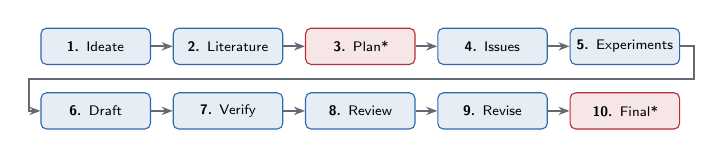
\begin{tikzpicture}[
  font=\sffamily\tiny,
  ph/.style={draw=gateblue, fill=gateblue!12, rounded corners=2pt,
             text width=1.32cm, align=center, minimum height=0.46cm, inner sep=1pt},
  hu/.style={draw=gatered, fill=gatered!12, rounded corners=2pt,
             text width=1.32cm, align=center, minimum height=0.46cm, inner sep=1pt},
  ar/.style={-{Stealth[length=1.4mm]}, gategray, thick}
]
% Row 1
\node[ph] (p1) at (0,0) {\textbf{1.} Ideate};
\node[ph] (p2) at (1.68,0) {\textbf{2.} Literature};
\node[hu] (p3) at (3.36,0) {\textbf{3.} Plan*};
\node[ph] (p4) at (5.04,0) {\textbf{4.} Issues};
\node[ph] (p5) at (6.72,0) {\textbf{5.} Experiments};

% Row 2
\node[ph] (p6) at (0,-0.82) {\textbf{6.} Draft};
\node[ph] (p7) at (1.68,-0.82) {\textbf{7.} Verify};
\node[ph] (p8) at (3.36,-0.82) {\textbf{8.} Review};
\node[ph] (p9) at (5.04,-0.82) {\textbf{9.} Revise};
\node[hu] (p10) at (6.72,-0.82) {\textbf{10.} Final*};

% Arrows Row 1
\draw[ar] (p1) -- (p2);
\draw[ar] (p2) -- (p3);
\draw[ar] (p3) -- (p4);
\draw[ar] (p4) -- (p5);

% Connector 5 to 6
\draw[ar] (p5.east) -- ++(0.18,0) -- ++(0,-0.41) -- (-0.85,-0.41) |- (p6.west);

% Arrows Row 2
\draw[ar] (p6) -- (p7);
\draw[ar] (p7) -- (p8);
\draw[ar] (p8) -- (p9);
\draw[ar] (p9) -- (p10);
\end{tikzpicture}
\caption{The ten workflow phases (* indicates mandatory human-in-the-loop sign-off; red phases cannot close autonomously; non-linear re-entry is supported).}
\label{fig:gates}
\end{figure}

\begin{table}[t]
\centering
\caption{System Gate Inventory by Functional Category}
\label{tab:gates}
\renewcommand{\arraystretch}{0.98}
\setlength{\tabcolsep}{2.5pt}
\footnotesize
\begin{tabular}{@{}ll>{\raggedright\arraybackslash}p{3.8cm}c@{}}
\toprule
\textbf{Category} & \textbf{Gate Name} & \textbf{Target Invariant / Diagnostic} & \textbf{Type} \\
\midrule
\rowcolor{rowtint} \textbf{Workflow} & autopilot & Phase exit predicate holds & \badgeblock \\
\rowcolor{rowtint} & kickoff & Plan approved before issues & \badgeblock \\
\rowcolor{rowtint} & rebuttal gate & Review feedback itemized & \badgeblock \\
\midrule
\textbf{Citation} & verify citations & 3-layer lookup + review & \badgeblock \\
& citation style & Required schema metadata & \badgeblock \\
& BibTeX audit & Duplicates, years, recency & \badgeblock \\
& citation align & Sentence-abstract lexical overlap & \badgeadvise \\
\midrule
\rowcolor{rowtint} \textbf{Integrity} & data gate & Numbers match regenerated data & \badgeblock \\
\rowcolor{rowtint} & integrity gate & Claims, privacy, bibliography & \badgeblock \\
\rowcolor{rowtint} & claim registry & Assertion extraction worksheet & \badgeadvise \\
\rowcolor{rowtint} & prose diagnostic & Repetitive n-gram pattern density & \badgeadvise \\
\midrule
\textbf{Venue / Ops} & format gate & Page limit, sections, macros & \badgeblock \\
& anonymity & Author macros, URLs, emails & \badgeblock \\
& privacy scan & Sensitive secrets/keys in repo & \badgeblock \\
& portability & Cross-platform script sanity & \badgeblock \\
& venue rules & Sync with published CFP guide & \badgeblock \\
\bottomrule
\end{tabular}
\end{table}

\section{The Gate Model}
\label{sec:gates}

Fig.~\ref{fig:gates} shows the ten phases of the authoring workflow. What makes the model more than a diagram is that gate conditions are evaluated against physical repository files, not against anything the model says: \texttt{notes/research-question.md} must exist with non-empty content, the bibliography must meet the configured reference threshold without unresolved keys, and every task in the issues CSV must be complete with verified acceptance criteria.

When the agent requests a phase transition, the gate script inspects the filesystem for itself. If a predicate fails, the gate exits with status code 1 and prints the specific unmet prerequisite, so the agent (and the author) knows exactly what is missing rather than receiving a vague refusal. Real research does produce legitimate exceptions, so the system supports a manual override: passing \texttt{--force} with a required justification advances the phase, but the justification becomes a permanent, append-only record in the run journal:

\begin{center}
\vspace{-3pt}
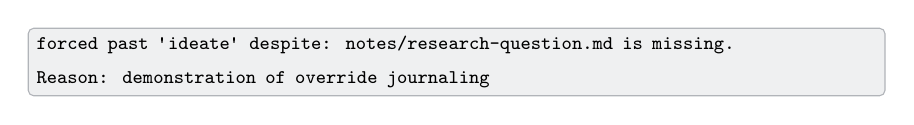
\begin{tikzpicture}
\node[draw=gategray!50, fill=gategray!10, rounded corners=2pt, inner sep=3pt, text width=0.88\columnwidth] {
\scriptsize\ttfamily\raggedright
forced past \textquotesingle ideate\textquotesingle\ despite: notes/research-question.md is missing.\\
Reason: demonstration of override journaling
};
\end{tikzpicture}
\vspace{-3pt}
\end{center}

Because journal entries are append-only through the CameraReady CLI state machine and cannot be purged via standard commands, every deviation stays visible forever. Table~\ref{tab:gates} summarizes the full gate inventory across all functional categories.

\section{Verification Mechanisms}
\label{sec:verify}

\subsection{The citation path}
Fig.~\ref{fig:cite} shows how bibliographic entries reach \texttt{ref.bib}, and just as importantly, how they cannot. The agent is free to formulate search queries, but the CLI toolchain offers no programmatic path for injecting raw BibTeX. Title queries go to DBLP and CrossRef, identifier queries to arXiv, and whatever comes back is normalized into a local SQLite registry before export. When a lookup fails, \texttt{fetch\_bibtex.py} exits cleanly with status 0 but emits an explicit \textsc{[verify]} marker and zero BibTeX records: the miss is recorded, not papered over. Enforcement happens downstream. Gates such as \texttt{verify\_citations.py}, \texttt{integrity\_gate.py}, and \texttt{arxiv\_package.py} scan \texttt{ref.bib} and halt with exit code 1 the moment they find an unresolved \textsc{[verify]} tag, so a draft containing an unverifiable reference cannot reach the packaging stage.

\begin{figure}[t]
\centering
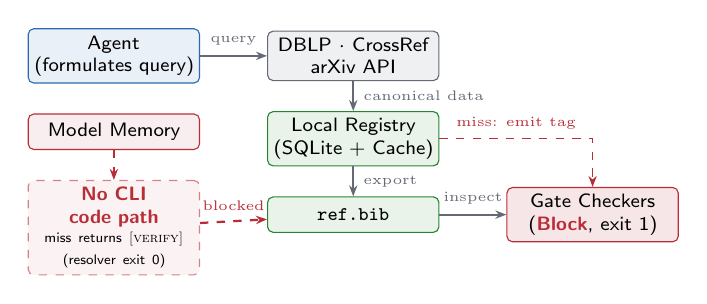
\begin{tikzpicture}[
  font=\sffamily\scriptsize,
  b/.style={draw, rounded corners=2pt, align=center, inner sep=2.5pt,
            minimum height=0.45cm, text width=2.0cm},
  ar/.style={-{Stealth[length=1.4mm]}, thick, gategray}
]
\node[b, draw=gateblue, fill=gateblue!10] (agent) {Agent\\(formulates query)};
\node[b, draw=gategray, fill=gategray!10, right=0.85cm of agent] (api) {DBLP $\cdot$ CrossRef\\arXiv API};
\node[b, draw=gategreen, fill=gategreen!10, below=0.38cm of api] (reg) {Local Registry\\(SQLite + Cache)};
\node[b, draw=gategreen, fill=gategreen!10, below=0.38cm of reg] (bib) {\texttt{ref.bib}};
\node[b, draw=gatered, fill=gatered!8, below=0.38cm of agent] (mem) {Model Memory};
\node[b, draw=gatered!60, fill=gatered!6, dashed, below=0.38cm of mem] (forbid) {%
  \textcolor{gatered}{\textbf{No CLI code path}}\\[1pt]
  \tiny miss returns \textsc{[verify]}\\(resolver exit 0)};
\node[b, draw=gatered, fill=gatered!12, right=0.85cm of bib] (gate) {Gate Checkers\\(\badgeblock, exit 1)};

\draw[ar] (agent) -- node[above, font=\tiny] {query} (api);
\draw[ar] (api) -- node[right, font=\tiny] {canonical data} (reg);
\draw[ar] (reg) -- node[right, font=\tiny] {export} (bib);
\draw[ar] (bib) -- node[above, font=\tiny] {inspect} (gate);

\draw[gatered, dashed, thick, -{Stealth[length=1.4mm]}] (mem) -- (forbid);
\draw[gatered, dashed, thick, -{Stealth[length=1.4mm]}] (forbid) -- node[above, font=\tiny, text=gatered] {blocked} (bib);

\draw[-{Stealth[length=1.4mm]}, dashed, gatered] (reg.east) -| node[pos=0.25, above, font=\tiny] {miss: emit tag} (gate.north);
\end{tikzpicture}
\caption{Bibliographic dataflow and trust boundary: The dashed path from model memory to \texttt{ref.bib} is absent from the CLI toolchain. Query misses emit \textsc{[verify]} tags (resolver exit 0), which are subsequently trapped by downstream blocking gates (exit 1).}
\label{fig:cite}
\end{figure}

\subsection{Resilience to external service disruptions}
Canonical registries are web services, and web services go down. Lookups therefore route through a persistent local cache indexed by query hash, so previously resolved citations survive API outages and rate limits. Fully network-isolated settings can point the tool at an offline JSON Lines corpus of pre-indexed papers via \texttt{--offline}. Cached records only ever corroborate citations that were verified when first fetched; a query with no cached or indexed answer yields an unverified marker, never a fabricated entry.

\subsection{Reconciling empirical data and reported metrics}
Numbers drift the same way citations do: a table is regenerated, the prose keeps yesterday's value, and nobody notices. The data gate closes this hole by binding each LaTeX table and figure to the data-generation script that produced it. When the gate runs, it re-executes the script, extracts the numerical tokens in the associated float, and checks that the reported numbers match the regenerated outputs within numerical tolerance, ignoring formatting numerals. A number the analysis does not produce fails the gate.

\subsection{Semantic citation alignment}
Some citation errors are subtler than fabrication: the cited paper exists but does not actually support the claim, making it a real reference acting as a false witness. The alignment checker addresses this by computing lexical and TF-IDF overlap between each citing sentence and its cited abstract. As an advisory diagnostic (\badgeadvise), it ranks the weakest pairings for the author to read rather than pretending to judge conceptual validity automatically.

\subsection{Claim extraction, prose diagnostics, and packaging}
Before packaging, the claim extractor parses the manuscript into a structured registry of factual assertions, and the integrity gate requires explicit human sign-off on every claim before the paper can ship. Prose diagnostics evaluate repetitive n-grams informatively, without blocking compilation. On the venue side, the format gate validates page limits and required sections, the anonymity checker flags author identifiers for double-blind submissions, and the packaging script bundles verified sources with inlined bibliographies into an arXiv-ready archive.

\section{Software Verification and Self-Application}
\label{sec:eval}

Evaluations ran on a Windows 10 workstation (build 10.0.19045, Python 3.13.9, MiKTeX); all reproduction commands and raw outputs are documented in \path{notes/experiment-results.md}. We assess CameraReady four ways: software verification of the implementation itself (545 unit tests across 34 modules), synthetic negative-control fault injections, an operational comparison of bibliographic provenance under live API conditions, and an end-to-end case study in which this very paper was written with the framework. Gate correctness is evaluated under injected faults; controlled comparison protocols against ungated agent baselines remain future work.

\begin{table}[t]
\centering
\caption{Negative Control Interceptions under Fault Injection}
\label{tab:neg}
\renewcommand{\arraystretch}{0.88}
\setlength{\tabcolsep}{2.5pt}
\scriptsize
\begin{tabular}{@{} >{\raggedright\arraybackslash}p{2.65cm} >{\raggedright\arraybackslash}p{4.25cm} c @{}}
\toprule
\textbf{Injected Fault Condition} & \textbf{Gate Diagnostic / Interception} & \textbf{Exit} \\
\midrule
\rowcolor{rowtint} Ideate without RQ & Flags missing \texttt{research-question.md} & \textcolor{gatered}{\codeexit{1}} \\
Kickoff without approval & Halts: plan approval checkbox unmarked & \textcolor{gatered}{\codeexit{1}} \\
\rowcolor{rowtint} Forced override w/ reason & Advances phase, logs rationale to journal & \textcolor{gategreen}{\codeexit{0}} \\
Missing IEEE \texttt{journal} & Rejects entry: mandatory key missing & \textcolor{gatered}{\codeexit{1}} \\
\rowcolor{rowtint} Signed paper anonymity & Flags 2 author macros, 1 URL (3 blockers) & \textcolor{gatered}{\codeexit{1}} \\
NeurIPS format breach & Flags missing sections and style & \textcolor{gatered}{\codeexit{1}} \\
\rowcolor{rowtint} Unadjudicated claims & Halts packaging: claim registry unapproved & \textcolor{gatered}{\codeexit{1}} \\
Fabricated paper title & Emits \textsc{[verify]}; 0 BibTeX (resolver 0; gate 1) & \textcolor{gategreen}{\codeexit{0}} \\
\rowcolor{rowtint} Mismatched table numbers & Traps discrepancy between prose and data & \textcolor{gatered}{\codeexit{1}} \\
Failing analysis script & Catches non-zero pipeline exit code & \textcolor{gatered}{\codeexit{1}} \\
\rowcolor{rowtint} Untracked rebuttal point & Halts: unmapped reviewer item & \textcolor{gatered}{\codeexit{1}} \\
Stale venue page limits & Catches outdated page count constraint & \textcolor{gatered}{\codeexit{1}} \\
\bottomrule
\end{tabular}
\end{table}

\begin{table}[t]
\centering
\caption{Three-Layer Bibliographic Verification Stability Across Six Remote Lookup Runs (Skipped denotes transient remote lookup throttling, not hallucination; union reflects distinct entries verified across runs).}
\label{tab:verify}
\renewcommand{\arraystretch}{0.88}
\setlength{\tabcolsep}{3.2pt}
\scriptsize
\begin{tabular}{@{}lcccc@{}}
\toprule
\textbf{Run} & \textbf{Verified} & \textbf{Suspicious} & \shortstack{\textbf{Hallucination}\\\scriptsize\textbf{Verdict}} & \shortstack{\textbf{Skipped}\\\scriptsize(Throttled / 429)} \\
\midrule
\rowcolor{rowtint} Run 1 & 39 & 0 & 0 & 6 \\
Run 2 & 38 & 0 & 0 & 7 \\
\rowcolor{rowtint} Run 3 & 41 & 0 & 0 & 4 \\
Run 4 & 38 & 0 & 0 & 7 \\
\rowcolor{rowtint} Run 5 & 45 & 0 & 0 & 0 \\
Run 6 & 45 & 0 & 0 & 0 \\
\midrule
\rowcolor{gateblue!12} \textbf{Union (1--6)} & \textbf{45} & \textbf{0} & \textbf{0} & \textbf{0 (complete)} \\
\bottomrule
\end{tabular}
\end{table}

\subsection{Unit verification and gate determinism}
The test suite spans 545 unit tests across 34 modules and completes in 48.87\,s with a 100\% pass rate. Continuous integration validates every commit across a 3-OS (Ubuntu, macOS, Windows) $\times$ 2-Python-version matrix with CLI smoke tests. The portability checker verified zero OS-specific assumptions across 220 files in \texttt{--docs} mode (102 scripts/tests, 118 docs), and the specification validator reported zero configuration warnings. Of the framework's 68 scripts, 65 are standalone CLI entry points and all 65 implement fail-stop non-zero exit codes; the remaining 3 are library modules imported by other scripts. The worked example compiles in 5.8\,s.

\subsection{Gate enforcement under negative controls}
We deliberately broke things on purpose to see whether the gates would notice. Twelve synthetic negative-control fixtures represent intentional violations of each gate's invariant (Table~\ref{tab:neg}); in every blocking case, the gate intercepted the non-compliant artifact and exited with status 1. Fed a fabricated title (``Gated Diffusion Transformers for Bibliographic Provenance Repair''), the resolver emitted an unresolved marker with zero BibTeX records rather than an entry. The data gate likewise intercepted an injected discrepancy (0.88 reported vs. 0.71 produced).

\subsection{Heuristic checker refinements}
The heuristics improved through use. Early claim extractors tokenized raw LaTeX markup into 48 noisy claims, one of which was a vector graphic; an AST cleaning pre-pass reduced this to 26 substantive assertions. Likewise, moving prose-logic checks to whole-document TF-IDF cosine similarity cut false-positive topical-disconnect warnings on this manuscript from 14 to 1.

\subsection{Provenance by construction vs. post-hoc screening}
In this case study, all 45 cited references were resolved via canonical arXiv queries and exported into \texttt{ref.bib}, with their persistent identifiers recorded in \path{citation-provenance.jsonl}. To test how that record holds up, we ran the three-layer verifier six times one afternoon under normal network conditions (Table~\ref{tab:verify}). No identity-level fabricated bibliographic records were observed under the stated registry criterion, but verified entries fluctuated between 38 and 45 purely because of transient upstream throttling (recorded in \path{notes/experiment-results.md}). Tested with three fabricated citations lacking identifiers, the verifier returned skipped rather than hallucination verdicts. Declining to guess is the right call, but an inconclusive verdict provides no safety guarantee, and this is exactly the gap that persisting canonical provenance in SQLite at ingestion time closes: the workflow does not have to re-resolve remotely what it already proved locally.

\subsection{Dogfooding self-application case study}
Finally, we used CameraReady to write the paper you are reading. The manuscript went end to end through ideation, literature gathering, plan approval, issues tracking (38 to 45 tasks), experiments, and drafting. During review, the rebuttal gate intercepted five unaddressed comments and mapped them automatically to tracked issues via \texttt{--emit-issues}. One manual override was exercised during drafting, when 16 presentation tasks were skipped; the transition and its rationale were permanently recorded in the run journal, exactly as P2 and P5 promise.

\section{Discussion, Limitations, and Future Work}
\label{sec:discuss}

\noindent\textbf{Validity, trust, and bounds.} CameraReady enforces syntactic and bibliographic invariants; judging scientific novelty or conceptual validity remains the author's responsibility~\cite{miyai2026paper}. The framework assumes a cooperative agent, so isolation against untrusted shell agents requires OS-level sandboxing. Textual heuristics assist rather than decide, and local SQLite caching mitigates, though does not eliminate, dependence on external APIs.\\
\noindent\textbf{Controlled benchmarking and future work.} This report verifies gate correctness under synthetic fault injection, but controlled empirical benchmarking of authoring error rates against unconstrained baselines (formalized in \texttt{benchmark\_compare.py}) remains future work, as do neural entailment for citation alignment and containerized execution recipes.\\
\noindent\textbf{Generative AI disclosure.} This paper was written using CameraReady, which orchestrates an LLM agent (Claude 3.5/4 Sonnet and Opus, Anthropic) through the ten-phase pipeline described above. The agent was used for literature query formulation, section drafting, and iterative revision under gate supervision. All factual claims, experimental measurements, citation selections, and the decision to submit were reviewed and approved by the human author. Bibliographic entries were resolved exclusively through registry APIs (arXiv, DBLP, CrossRef) as described in Section~\ref{sec:verify}; no reference originates from model parametric memory.\par\vspace{2pt}
{\footnotesize\raggedright\noindent\textbf{Data and code availability.} Open source (MIT) at \url{https://github.com/e96031413/camera-ready} (tag \texttt{v0.2.0}, commit \texttt{29a8fdb6a539f4b4e7cfb86988e6691714146e69}). Reproduction commands and raw outputs: \path{notes/experiment-results.md}; reference provenance records: \path{citation-provenance.jsonl}.\par}

\section{Conclusion}

Citation hallucination, numerical drift, and formatting violations are not exotic failure modes; they are what unconstrained authoring agents do by default. CameraReady's claim is that the mechanically checkable subset of manuscript integrity can be enforced deterministically, by building verification gates into the authoring lifecycle rather than bolting detection on afterward. In practice that means three things: the model's memory never touches the bibliography, phase transitions happen only when the filesystem says so, and venue rules live in schemas rather than prompts. What requires judgment is flagged for the author, what requires scholarship is signed off by the author, and everything in between is checked by scripts that refuse to stay silent.
\newpage
\label{ReferencesStart}
\IEEEtriggeratref{20}
\bibliographystyle{ieeetr}
\bibliography{ref}

\end{document}
